\documentclass[../fem.tex]{subfiles}

\begin{document}
\section{Localization}%
\label{sec:localization}

While it is possible to find the elements of the matricies in
(\ref{eq:mat_rep}) on the global domain, this proves to be exedingly difficult,
and so we will use a more generalizable method. Since we are able to selece our
basis function $\varphi_j$ we can carefully construct a set of basis functions
such that it is possible to split the domain into discrete elements. Where each
element is a mutualy exclusive subset of the domain. We can then implement a
generalization to construct the system of equations for each element. Then
using an algorithm we combine each system of equations for each element to
construct the global matricies, which can then be solved for our approximation.

We discretize the domain $\Omega$ into $N$ triangles. This process of
constructing the triangular decomposition of the domain is detailed in the
numerical computation section \ref{sec:mesh_generation},  Mesh Generation. For
now we assume that we have constructed a mesh of $N$ triangles, and we denote
the each of these triangles $E_e$, where $e=1,\ldots,N$. We then also define
the triangle verticies to be labeled $E_e^{(i)}$ where $i=1,2,3$.

In 1D this step is fairly trivial as all elements have the exact same
dimesnions, but in our 2D implementation, each element can have variable shapes
and sizes. Inorder to resolve this we construct a master space.

\subsection{Master Space}%
\label{sub:master_space}

The master space is a domain that we construct inorder to simplify the
construction of our local approximations. For our situation with a triangular
element we construct our global space such that the verticies of a triangle lie
on the points $(1,0,0)$, $(0,1,0)$, and $(0,,01)$. Then for each element in our
mesh, we construct the transformation matrix $T$ to transform between master
space and element space. We define our master element to be $\hat{E}$. An image
of this master element can be seen in figure \ref{fig:master_element}.

\begin{Figure}
   \begin{center}
     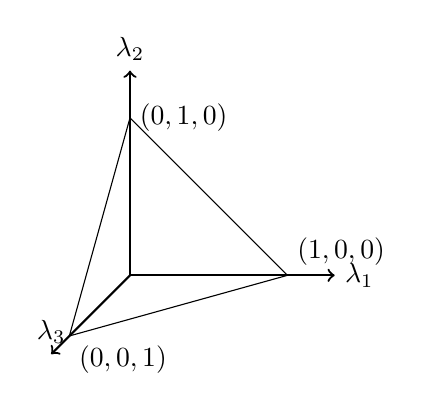
\begin{tikzpicture}[scale=2]
        \draw[thick,->] (0,0,0) -- (1.3,0,0) node[right]{$\lambda_1$};
        \draw[thick,->] (0,0,0) -- (0,1.3,0) node[above]{$\lambda_2$};
        \draw[thick,->] (0,0,0) -- (0,0,1.3) node[above]{$\lambda_3$};
        \draw (1,0,0) node[above right]{$(1,0,0)$}-- (0,1,0)
        node[right]{$(0,1,0)$} -- (0,0,1) node[below right]{$(0,0,1)$}-- cycle;
      \end{tikzpicture}
   \end{center}
   \captionof{figure}{Master element $\hat{E}$.}\label{fig:master_element}
\end{Figure}

This master element is in what is called a Barycentric coordinate system.
Conversion from our trilinear coordinates to the Barycentric coordinates can be
done by using the following equations

\begin{align*}
  \lambda_1 &=
  \frac{\left(E^2_y-E^3_y\right)\left(x-E^3_x\right)+\left(E^3_x-E^2_x\right)\left(y-E^3_y\right)}{\left(E^2_y-E^3_y\right)\left(E^1_x-E^3_x\right)+\left(E^3_x-E^2_x\right)\left(E^1_y-E^3_y\right)}\\
  \lambda_2 &=
  \frac{\left(E^3_y-E^1_y\right)\left(x-E^3_x\right)+\left(E^1_x-E^3_x\right)\left(y-E^3_y\right)}{\left(E^2_y-E^3_y\right)\left(E^1_x-E^3_x\right)+\left(E^3_x-E^2_x\right)\left(E^1_y-E^3_y\right)}\\
  \lambda_3 &= 1-\lambda_1-\lambda_2.
\end{align*}

Where $E^i_x$ is the $x$ component of the $i$th vertex of the element, the same
applies for the $y$ component. $x$, and $y$ is the $x$ and $y$ component of the
point in the triangle that we want to convert to the Barycentric coordinates.

Converting from Barycentric coordinates to trilinear coordinates uses the
following equations

\begin{align*}
  x &= \lambda_1 E^1_x+\lambda_2 E^2_x + \lambda_3 E^3_x\\
  y &= \lambda_1 E^1_y +\lambda_2 E^2_y + \lambda_3 E^3_y
\end{align*}

\subsection{Local Basis}%
\label{sub:local_basis}


We want to construct three local basis functions, that are defined only for the
current element. We aim to construct three local basis functions functions
$\varphi_1^{(e)}$, $\varphi_2^{(e)}$, and $\varphi_3^{(e)}$.  Each shape
function should be linear, such that at its cooresponding vertex the local
basis function is $1$ and at the other verticies the function should evaluate
to $0$.

\otodo{Provide better reasoning for this neccesity.}

Conviniently this is exactly what the barycentric coordinates of the master
element provide us with, thus we define our local basis functions to be 

\begin{align}\label{eq:local_basis}
  &\resizebox{\columnwidth}{!}{$
    \varphi_1^{(e)}=
  \frac{\left(E^{(e)}_{2_y}-E^{(e)}_{3_y}\right)\left(x-E^{(e)}_{3_x}\right)+\left(E^{(e)}_{3_x}-E^{(e)}_{2_x}\right)\left(y-E^{(e)}_{3_y}\right)}{\left(E^{(e)}_{2_y}-E^{(e)}_{3_y}\right)\left(E^{(e)}_{1_x}-E^{(e)}_{3_x}\right)+\left(E^{(e)}_{3_x}-E^{(e)}_{2_x}\right)\left(E^{(e)}_{1_y}-E^{(e)}_{3_y}\right)}
  $}\\
  &\resizebox{\columnwidth}{!}{$
    \varphi_2^{(e)}=
    \frac{\left(E^{(e)}_{3_y}-E^{(e)}_{1_y}\right)\left(x-E^{(e)}_{3_x}\right)+\left(E^{(e)}_{1_x}-E^{(e)}_{3_x}\right)\left(y-E^{(e)}_{3_y}\right)}{\left(E^{(e)}_{2_y}-E^{(e)}_{3_y}\right)\left(E^{(e)}_{1_x}-E^{(e)}_{3_x}\right)+\left(E^{(e)}_{3_x}-E^{(e)}_{2_x}\right)\left(E^{(e)}_{1_y}-E^{(e)}_{3_y}\right)}
  $}\\
  &\varphi_3^{(e)}=1-\varphi_1^{(e)}-\varphi_2^{(e)}
\end{align}

Thus for every element, there are three local basis functions. A plot of these
local basis functions is shown in figure \ref{fig:local_basis}.

\begin{Figure}
   \begin{center}
     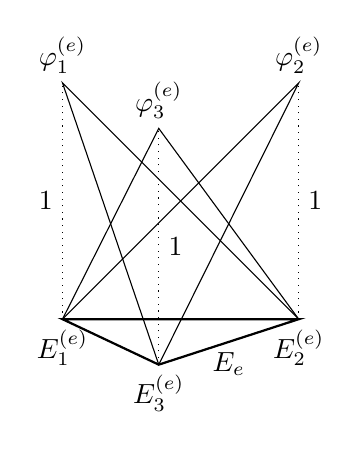
\begin{tikzpicture}[scale=3]
       \draw[thick] (0,0,0)node[below]{$E^{(e)}_1$} --
         (1,0,0)node[below]{$E^{(e)}_2$}
         --node[below]{$E_e$} (0.6, 0, 0.5)node[below]{$E^{(e)}_3$} -- cycle;
       \draw (0,1,0)node[above]{$\varphi_1^{(e)}$}  -- (1,0,0) -- (0.6, 0, 0.5)-- cycle;
       \draw (0,0,0) -- (1,1,0)node[above]{$\varphi_2^{(e)}$}  -- (0.6, 0, 0.5)-- cycle;
       \draw (0,0,0) -- (1,0,0) -- (0.6, 1, 0.5)node[above]{$\varphi_3^{(e)}$} -- cycle;
       \draw[dotted] (0,0,0) --node[left]{$1$} (0,1,0);
       \draw[dotted] (1,0,0) --node[right]{$1$} (1,1,0);
       \draw[dotted] (0.6,0,0.5) --node[right]{$1$} (0.6,1,0.5);
      \end{tikzpicture}
   \end{center}
   \captionof{figure}{Plot of local basis function $\varphi_1^{(e)}$,
   $\varphi_2^{(e)}$, and $\varphi_3^{(e)}$.}\label{fig:local_basis}
\end{Figure}

\subsection{Global Basis}%
\label{sub:global_basis}

We now construct the global basis functions. We chose the global basis
functions to be associated with a vertex of the mesh, thus for $N$ mesh
verticies are $N$ global basis functions. We want the global basis functions be
be $1$ at their associated vertex, and at all other mesh verticies the global
basis function should be $0$. Inorder to achive this we construct the global
basis functions as a piecewise combination of $n$ different local basis
functions, where $n$ is the number of elements that share a givin vertex. There
is not a simple mathematical expression for the global basis function, as it
greatly depends on the triangular mesh, and the current vertex index. However,
an example of a global basis function is shown in figure
\ref{fig:global_basis}.

\begin{Figure}
   \begin{center}
      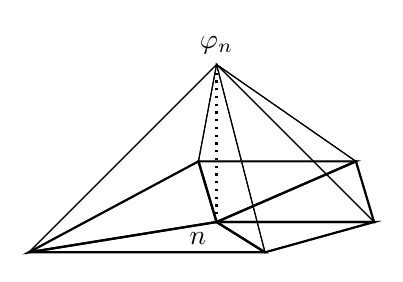
\begin{tikzpicture}

        % \draw[fill=gray] (0,2,0) -- (1,0,-2) -- (2,0,0) -- cycle;
        % \draw[fill=gray] (0,2,0) -- (2,0,0) -- (1,0,1) -- cycle;
        % \draw[fill=gray] (0,2,0) -- (1,0,1) -- (-2,0,1) -- cycle;
        % \draw[fill=gray] (0,2,0) -- (-2,0,1) -- (-1,0,-2) -- cycle;
        % \draw[fill=gray] (0,2,0) -- (-1,0,-2) -- (1,0,-2) -- cycle;

        \draw (0,2,0) -- (1,0,-2) -- (2,0,0) -- cycle;
        \draw (0,2,0) -- (2,0,0) -- (1,0,1) -- cycle;
        \draw (0,2,0) -- (1,0,1) -- (-2,0,1) -- cycle;
        \draw (0,2,0) -- (-2,0,1) -- (-1,0,-2) -- cycle;
        \draw (0,2,0) -- (-1,0,-2) -- (1,0,-2) -- cycle;

        \draw[thick] (0,0,0) -- (1,0,-2) -- (2,0,0) -- cycle;
        \draw[thick] (0,0,0) -- (2,0,0) -- (1,0,1) -- cycle;
        \draw[thick] (0,0,0) -- (1,0,1) -- (-2,0,1) -- cycle;
        \draw[thick] (0,0,0) -- (-2,0,1) -- (-1,0,-2) -- cycle;
        \draw[thick] (0,0,0) -- (-1,0,-2) -- (1,0,-2) -- cycle;

        \draw[dotted, thick] (0,0,0)node[below left]{$n$} -- (0,2,0) node[above]{$\varphi_n$};

      \end{tikzpicture}
   \end{center}
   \captionof{figure}{Gloabal basis function.}\label{fig:global_basis}
\end{Figure}

\end{document}
